\chapter{Simulation déterministe}

Dans un premier temps, nous avons pu analyser une simulation déterministe entre 2017 et 2023. Cette simulation nous permettra d'étudier les phénomènes de plus longue durée ainsi que d'avoir une base de comparaison une fois les ensembles effectués. Les données sont sauvegardées toutes les 24 heures ce qui permettra de construire des séries temporelles par la suite.

\section{Traceurs passifs}
Il est possible d'afficher les cartes de chacun de ces traceurs qui sont la température de surface, la salinité de surface et la hauteur de la surface libre en \autoref{fig:annu SS}.
\begin{figure}[h]
	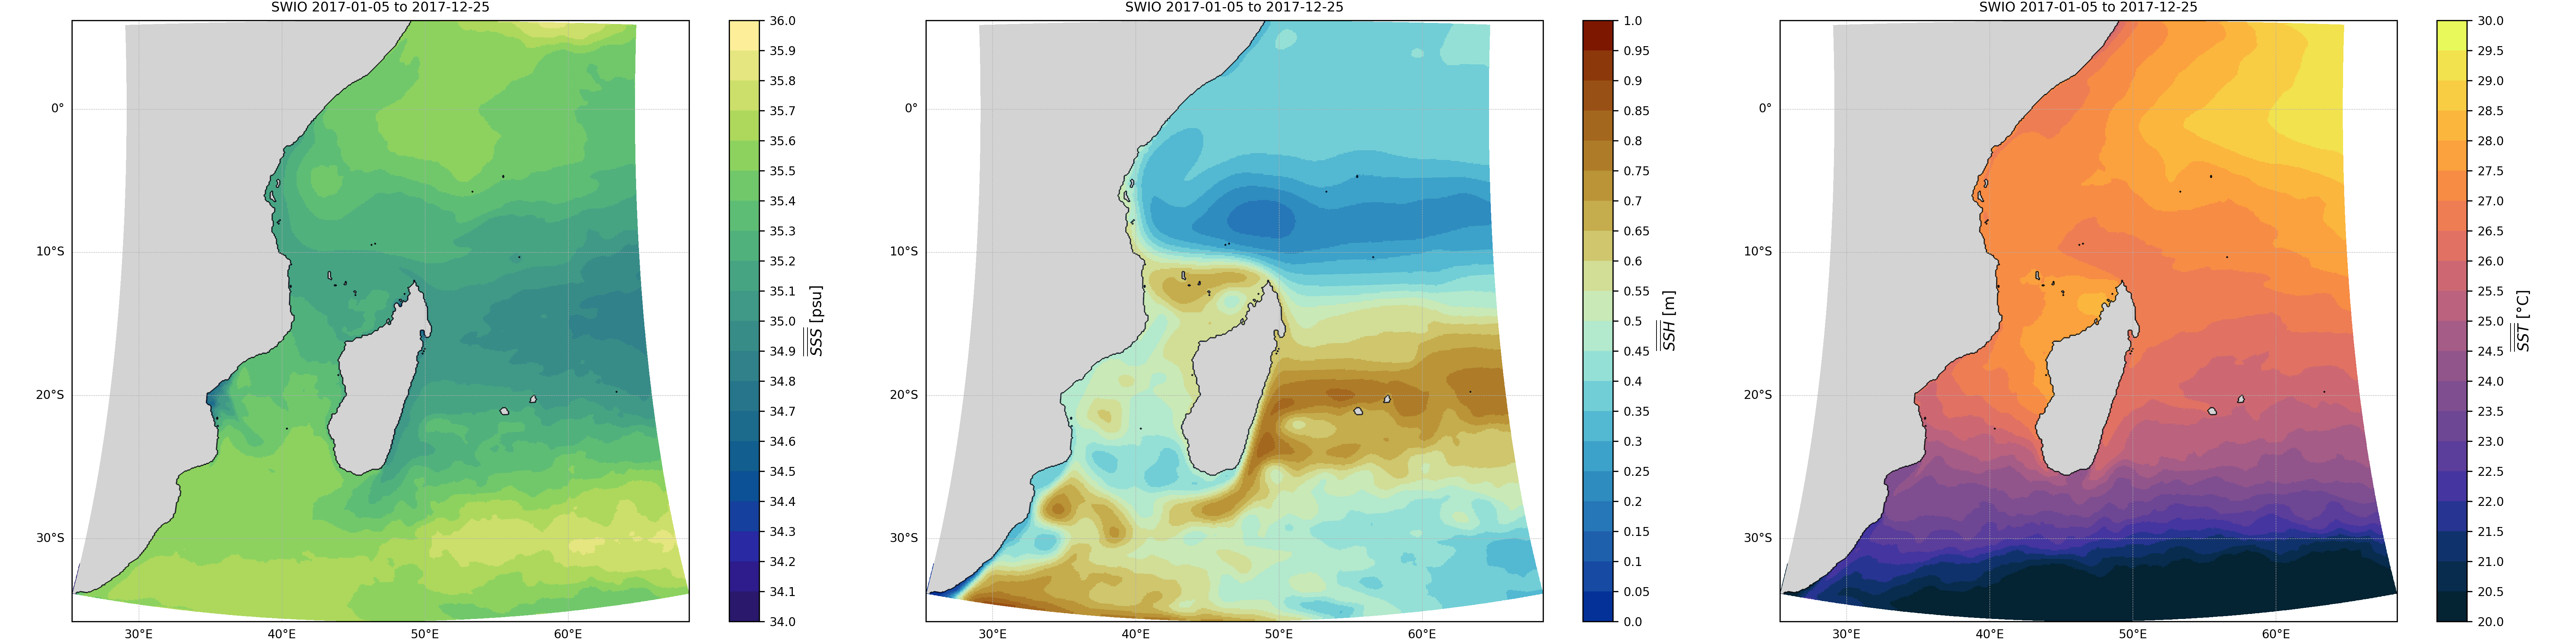
\includegraphics[width=\textwidth]{Figures/sea_surface_2017.png}
	\caption{Carte des valeurs de surface pour l'année 2017 - De gauche à droite: Salinité, Surface libre, Température}
	\label{fig:annu SS}
\end{figure}

On constate une salinité plus faible au niveau de l'embouchure du fleuve Pungue (35°E 20°S environ), cette différence ne sera pas visible sur les années suivantes. Elle est due aux champ initial qui prend en compte l'injection des eaux fluviales contrairement au modèle qui ne les prend pas en compte sur cette simulation. 

Ces figures nous permettent de visualiser les comportements moyens des masses d'eaux ainsi que leur caractéristiques. Ces données nous serviront également à calculer les anomalies annuelles (SSA,SLA,STA) en \autoref{fig:annu SA}. 

\begin{figure}[h]
	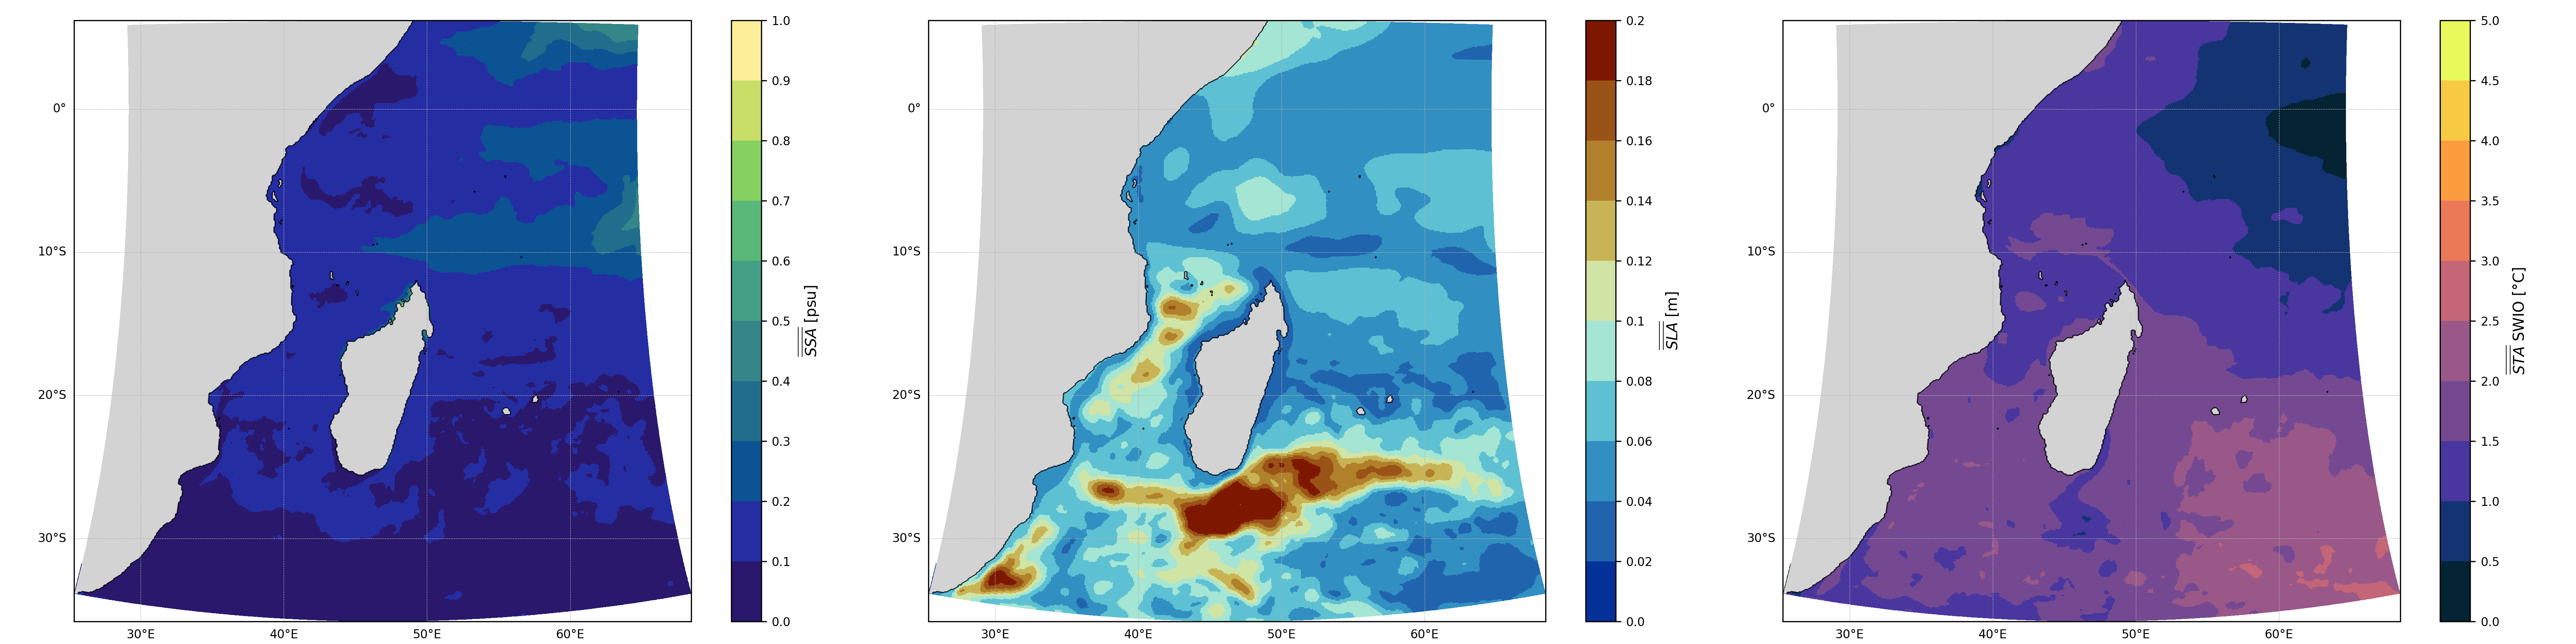
\includegraphics[width=\textwidth]{Figures/sea_anomaly_annual_2019.png}
	\caption{Carte des anomalies de surface pour l'année 2019 - De gauche à droite: Salinité, Surface libre, Température}
	\label{fig:annu SA}
\end{figure}
